\documentclass[a4paper,15pt]{article}
\usepackage[utf8]{inputenc}
\usepackage{graphicx}
\graphicspath{ {./images/} }

\title{Intelligent IoT Security using Fuzzy Optimum path forest classifier}
\author{Vignesh Raam S R }
\date{January 2023}


\begin{document}


\maketitle

\section*{Far Flew IoT}
\paragraph{
    In the Current world Scenario, each and everything we are looking for in one way or another has used up the IoT technology in it. From Fitness Bands to even auto-pilot Cars.
}


\section*{Need For Security}
\paragraph{
Now Think what if some stranger comes to get his hands over your Tesla's run time Data and manipulates those values and feeds it back!! Well, then you wouldn't even be alive. IoT Security is a must not just here but in many other cases like critical IoT tasks in the Military and Industry.
}


\section*{How To detect Intrusions ??}
\paragraph{
In the last decades, machine learning (ML) techniques have
been applied for Cyber-attack detection in IoT environments.
The objective of these works is to find solutions that
can prevent, detect, or mitigate attacks on this type of network.
There are several works have been done using machine learning algorithms
to build Intrusion Detection Systems (IDS)
}
\paragraph{}
\begin{enumerate}
    \item intrusion detection system based on
distributed machine learning using Blockchain technology.
    \item
    The classification technique - support vector machine (SVM) was trained using the datasets obtained from each of the nodes of the IoT network.
    \item IDS model based on DL and ML to overcome security
attacks in IoT networks, using K-Nearest Neighbor (KNN), and
Long Short-Term Memory (LSTM)
    \item Random Forest to select
important dataset features and Classification and Regression
Trees (CART) to classify different attack classes
    \item a model called Fuzzy Intrusion Detection
System for IoT Networks (FROST). FROST uses the basis of
fuzzy theory to make learning models more flexible, seeking
to improve performance in the classification of imprecise data.
    \item Fuzzy Optimum-Path Forest (Fuzzy OPF)  is a variant
of the OPF classifier designed as a pattern recognition
technique
\end{enumerate}
\section*{Fuzzy Optimum-path Forest Approach}
\paragraph{
 Firstly Fuzzy logic is where we have classified classes based Degree of Truth
 We try to apply that logic for all Required points. Each sample will have a value that will be calculated with the help of a function whose one Parameter is the density of the sample. The Forest is nothing but a Graph G(N, A).
}
\paragraph{\textbf{
where,
N is a grouping of Training class nodes and  A is a set of edges connecting the Nodes in N
}}
\paragraph{
The Grouping of the Training data into samples whose density is calculated using the below function
}
\paragraph{}
\Large p(s) = $\Sigma ( (\sqrt{1/2\Pi \psi ^2 k} )* exp -d^2(q,u) / 2 \psi ^2 ) $
\paragraph{}
\Large for all u $\epsilon$ A(q)

\paragraph{\textbf{
where A(q) is KNN of a sample q\\
$\psi$ = df/3 where  df is the highest\\ value between the edge of the graph
}}
\paragraph\Large{
For scaling the input values the algorithm uses of Fuzzy Membership whose function is given Below:
}
\paragraph{}
\Large{
    $F(q) = (1 -\sigma)*(P(q)-Pmin)/(Pmax-Pmin)  + \sigma $
}
\paragraph{
Now We also need a Path Cost function which is gonna say whether a path is present in the prototype data
The function for that is Below:
}
\paragraph{}
\Large
{

F max(u) = \[  \left\{
\begin{array}{ll}
      0 & if x\epsilon T \\
      + \infty & Otherwise \\
\end{array} 
\right. \]
}
\paragraph{}

\Large{

    Fmax($\phi$ * $<q,u>$)  = min(F(u) * max(p(q),d(q,u))) For all q$\epsilon$ N 
}
\section*{Proposed approach}
{
The Switch is the only way through which all the devices are connected Using that switch we can get the network traffic and give it to the intrusion monitor (Fuzzy OPF) . It detects the 
intrusion and alerts the user
}
\section*{
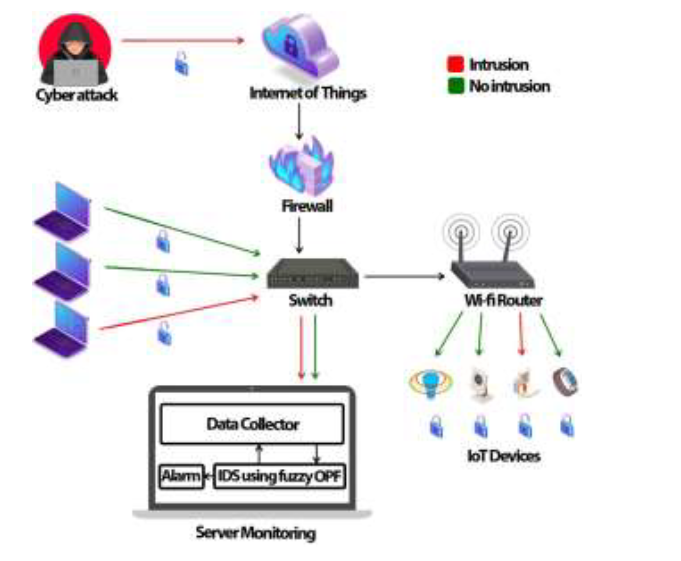
\includegraphics[width=15cm, height=10cm]{flowchart}
}
\paragraph{}
\section*{Conclusion}
\paragraph{
There using Fuzzy OPF we can find whether there is some sort of intrusion from the outside world and we lead a more secure privacy
Also, the if we see the Confusion Matrix of Fuzzy OPF we can see that it is Highly Accurate. Also If we want to we can do Hyper Parameter Tuning to further increase the result. But of course more accurate the Training data The Better Detection!!!
}
\section*{
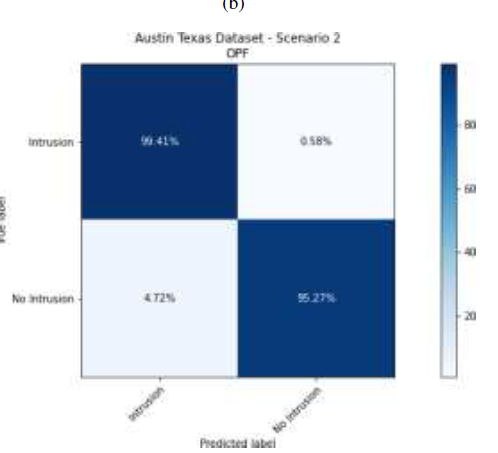
\includegraphics[width=15cm, height=10cm]{Confusion}
}
\end{document}
